\section{FFS - Forces on Fracture Surfaces}
\index{FFS Forces on Fracture Surfaces}
The FFS method (see chapter \ref{chap:NumPlatf:FFS}) was developed to simulate direct shear tests. To provide a tool for the project work and get things easier done a graphical user interface (GUI) was also created. The GUI simply calls all necessary functions by letting the user either fill form fields or choose input files from the working folder. The rock parameters and the conditions of the direct shear test with the normal stress levels and shear displacements have to be selected. If an experiment is simulated the lab results can be selected as a text file so a visual comparison is possible. The geometry has to be loaded as a point cloud or an artificial surface can be generated. With small modifications the code can do multiple executions using artificial surfaces.

The GUI can be found at \url{www.github.com/Poetschke/Ecodist/}. At github an executable is available which allows (after some installation) to test it without needing a Matlab licence.
The scheme of the FFS algorithm is illustrated in Fig. \ref{fig:AppendixFFSFigure}.

\begin{figure}[htp!]
\centering
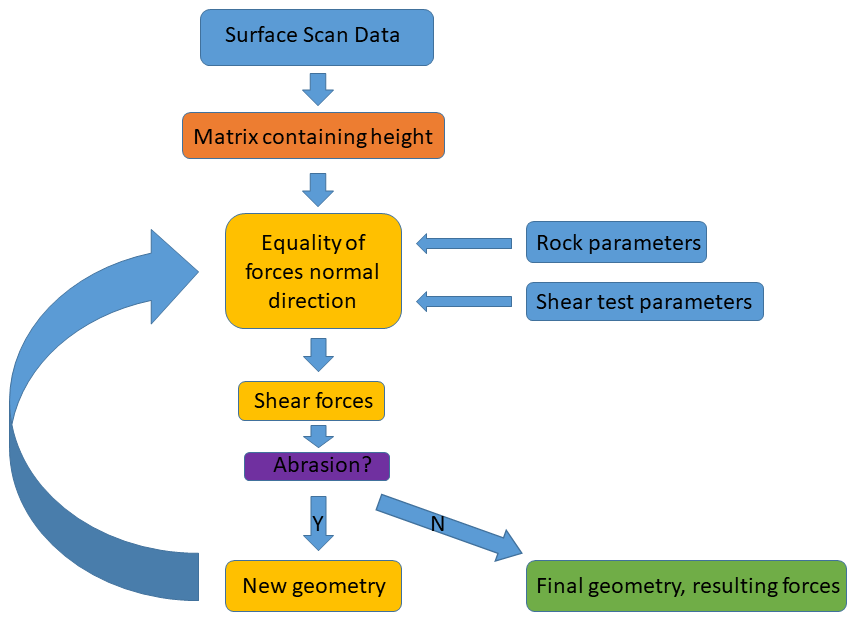
\includegraphics[width=0.9\textwidth]{figures/MEX7_Scheme.png}
\caption{Scheme of the FFS code.}
\label{fig:AppendixFFSFigure}
\end{figure}
